\documentclass[12pt]{article}
\usepackage{graphicx, geometry, hyperref} % Required for inserting images
\usepackage{physics,caption, amsmath, amsfonts, tikz, minted}
\usepackage{scalerel, cases, multirow, multicol}
\usepackage{tabularx}
\graphicspath{{images/}}
\hypersetup{colorlinks=true,citecolor=black,linkcolor=black,urlcolor=black}
\geometry{
a4paper,
total={170mm,257mm},
left=20mm,
top=20mm,
}
% \usepackage[table]{xcolor}
% \usepackage{eulervm}
% \usepackage{booktabs}


%-------------new commands----------------------
\newcommand{\bc}[1]{{\color{blue}{#1}}}
\newcommand{\red}[1]{{\color{red}{#1}}}
\begin{document}

\begin{center}
    \Large \bfseries{Weekly Report}
\end{center}

\begin{center}
    \Large \bfseries{CS3500: Operating Systems}
\end{center}


\begin{center}
    \Large \bfseries{Visualisation Tool for Process Scheduling}
\end{center}
\begin{center}
    \vspace{1.2cm}
    
\includegraphics[width=5cm]{logos and images/IIT_Madras_Logo.svg.png}

    \textbf{Computer Science and Engineering}
    \vspace{0.3cm}

    \textbf{Indian Institute of Technology  Madras}
    \vspace{0.3cm}

    \textbf{Jul - Nov 2024}
    \vspace{1.2cm}

    \noindent \textbf{Under the supervision}
    \vspace{0.2cm}

    \noindent \textbf{of}
    \vspace{0.2cm}

    \noindent\textbf{Prof. Janakiram D}
     \vspace{0.2cm}

    \noindent \textbf{submitted by}
    \vspace{0.3cm}

    \noindent \textbf{Team 8}
    \begin{multicols}{2}
        \begin{itemize}
            \item Anjali Samudrala (CS22B046)
            \item Chaitanya Sai Teja G (CS22B036)
            \item Jwala Likitha Reddy M (CS22B078)
            \item Karthikeya P (CS22B026)
            \item Naveen Koushik Reddy E (CS22B006)
            \item Navya Sree B (CS22B045)
            \item Rushi Babu G (CS22B040)
            \item Sravya Rangu (CS22B044)
            \item Yashwanth Sai P (CS22B002)
            \item Yaswanth Sai V (CS22B043)
        \end{itemize}
    \end{multicols}
    \vspace{0.5cm}

\end{center}
\clearpage

\section{Design Choices}
\subsection{Frontend}
We choose to use ReactJS for the frontend of our project. ReactJS is a JavaScript library that is used to build user interfaces. It is maintained by Facebook and a community of individual developers and companies. ReactJS is used for handling the view layer for web and mobile apps. ReactJS allows us to create reusable UI components. It is currently one of the most popular JavaScript libraries and has a strong foundation and large community behind it. We chose ReactJS because it is easy to learn and use, and it allows us to create a dynamic and interactive user interface.

\subsection{Backend}
We choose to use Flask for the backend of our project. Flask is a micro web framework written in Python. It is lightweight and easy to use. Flask is designed to make getting started quick and easy, with the ability to scale up to complex applications. We chose Flask because it is easy to learn and use, and it allows us to create a RESTful API for our project. Flask is also easy to deploy and maintain, which makes it a good choice for our project.

\subsection{Communication between Frontend and Backend}
We are using the socket framework to establish communication between the frontend and the backend. The socket framework allows us to establish a bidirectional communication channel between the client and the server. This allows us to send and receive data in real-time, which is important for our project. We are using the socket.io library for the frontend and the Flask-SocketIO library for the backend. These libraries make it easy to establish a socket connection between the client and the server and send and receive data in real-time.

\section{Plots}
\subsection{Top 5 High-Load Processes}
\begin{figure}[H]
    \centering
    \begin{minipage}{0.45\textwidth}
        \centering
        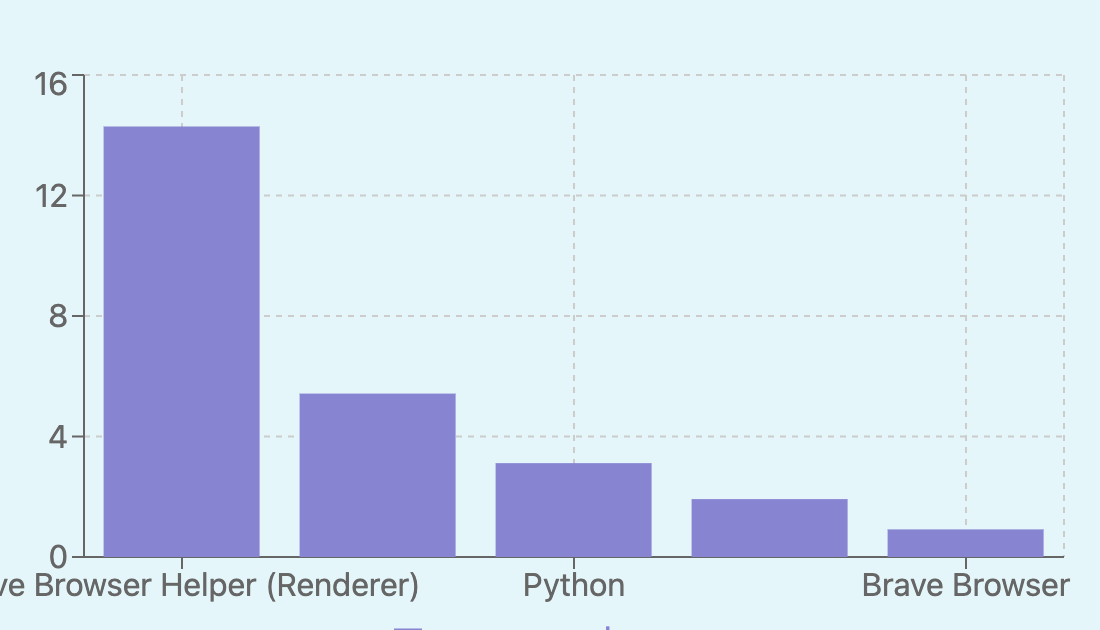
\includegraphics[width=\textwidth]{logos and images/top5_1.png}
    \end{minipage}
    \hfill
    \begin{minipage}{0.45\textwidth}
        \centering
        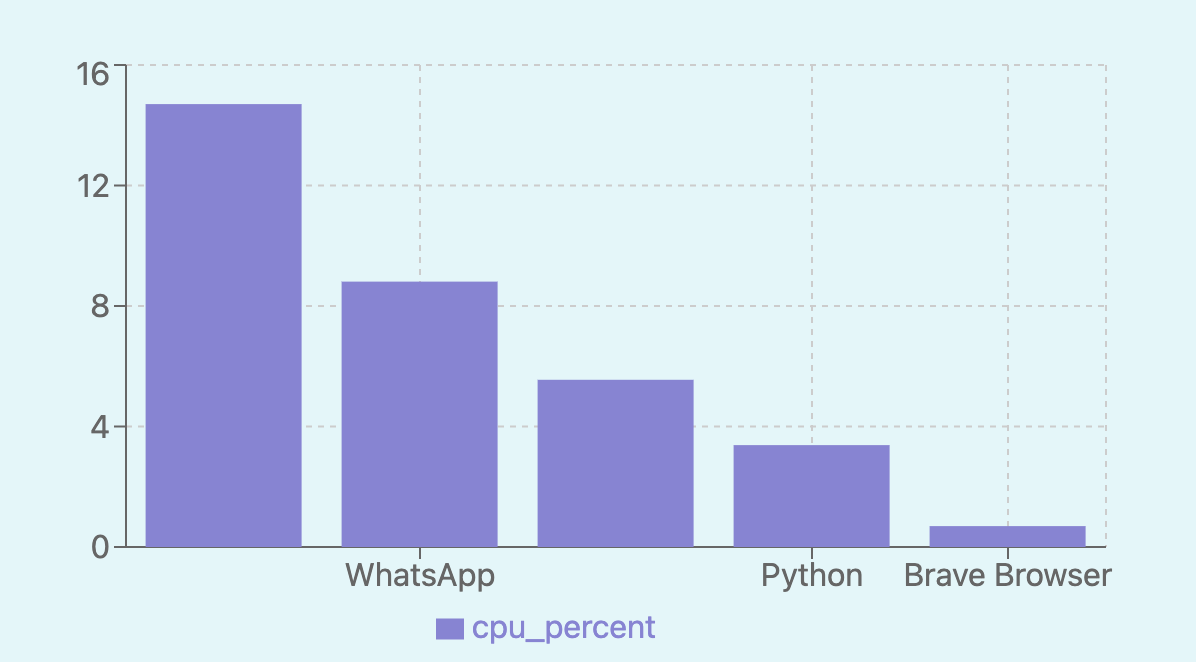
\includegraphics[width=\textwidth]{logos and images/top5_2.png}
    \end{minipage}
    \caption{Top 5 High-Load Processes at different time instances}
\end{figure}

The plot shows the top 5 high-load processes in the system. The x-axis represents the process ID, and the y-axis represents the \% CPU load of the process. The plot shows the CPU load at two different instances of the time. The plot is updated in real-time, so the user can see the CPU load of the top 5 high-load processes as it changes over time.
\end{document}